%&./out/hands-on-ml_slides_chapter-13-1st-half
% use precompiled file
%%%%%%%%%% ↑ EDIT FILE NAME ↑ %%%%%%%%%%

% @file           hands-on-ml_slides_chapter-13-1st-half.tex
% @brief          Template slides of beamer (LaTeX)
% @author         Kataoka Nagi
% @date           2021-05-13 00:17:45
% $Version:       1.0
% @par            History
%                 new file
% Copyright (c) 2021 Kataoka Nagi
% - This src is released under the MIT License, see LICENSE.

%%%%%%%%%%%%%%%%%%%%%%%%%%%%%%%%%%%%%%%%%%%%%%%%%%
%%%%%%%%%%%%%%%%%%%%%%%%%%%%%%%%%%%%%%%%%%%%%%%%%%

% \documentclass[dvipdfmx, 11pt]{beamer}^
% aspectratio = 43, 149, 169
% font size = 8pt, 9pt, 10pt, 11pt, 12pt, 14pt, 17pt, 20pt
% @see 「Beamer columns 環境で画像を配置するベストな方法」https://qiita.com/t_uda/items/8ef173eebf9827305135#3-columns-%E7%92%B0%E5%A2%83%E3%81%AE%E6%AD%A3%E3%81%97%E3%81%84%E4%BD%BF%E3%81%84%E6%96%B9
\PassOptionsToClass{hiresbb}{graphicx}
\documentclass[aspectratio=169, dvipdfmx, 14pt, xcolor={svgnames,dvipsnames}, t]{beamer}

%%%%%%%%%%%%%%%%%%%%%%%%%%%%%%%%%%%%%%%%%%%%%%%%%%

\usepackage{graphicx}
\newcommand{\thickhrulefill}{\leavevmode\leaders\hrule depth-1.2pt height 3.2pt\hfill\kern0pt}
\newcommand{\indicatewidth}[1]{\thickhrulefill{#1}\thickhrulefill}
\newlength{\mytotalwidth}
\mytotalwidth=\dimexpr\linewidth-5mm
\newlength{\mycolumnwidth}
\mycolumnwidth=\dimexpr\mytotalwidth-5mm

\usepackage{base_kataoka-nagi}
\usepackage{slides_kataoka-nagi}

%%%%%%%%%%%%%%%%%%%%%%%%%%%%%%%%%%%%%%%%%%%%%%%%%%

% precompile preamble from here.
% don't precompile with glossaries-env!
% type [eptex -ini -jobname="FILE_NAME" "&platex" mylatexformat.ltx FILE_NAME.tex] in cd
% @see 「beamerのコンパイル速度を上げる」 http://margaret-sdpara.blogspot.com/2019/11/beamer.html
\endofdump

% \usepackage{background}
\usepackage{wrapfig}

%%%%%%%%%%%%%%%%%%%%%%%%%%%%%%%%%%%%%%%%%%%%%%%%%%

% current build \begin{frame}[label=current]
% \includeonlyframes{current}

%%%%%%%%%%%%%%%%%%%%%%%%%%%%%%%%%%%%%%%%%%%%%%%%%%

\title[13章 前半 TFによるデータのロードと前処理]{scikit-learn、Keras、TensorFlowによる\\実践機械学習 第2版 第13章 前半\\
TensorFlowによるデータのロードと前処理}
\subtitle{データ工学研究室 輪読会}
\author[片岡 凪]{AL18036 片岡 凪}
% \institute[SIT]{芝浦工業大学 工学部 情報工学科 4年}
\institute[データ工学研究室 B4]{芝浦工業大学 工学部 情報工学科 4年}
\date{May 13, 2021}

%%%%%%%%%%%%%%%%%%%%%%%%%%%%%%%%%%%%%%%%%%%%%%%%%%

% tableofcontents
% LATEX Beamerの使い方 http://joker.hatenablog.com/entry/2014/10/18/222303
\AtBeginSection[]{
    \begin{frame}{目次}
        \tableofcontents[currentsection]
    \end{frame}
}

\AtBeginSubsection[]{
    \begin{frame}{目次}
        \tableofcontents[currentsubsection]
    \end{frame}
}

%%%%%%%%%%%%%%%%%%%%%%%%%%%%%%%%%%%%%%%%%%%%%%%%%%
%%%%%%%%%%%%%%%%%%%%%%%%%%%%%%%%%%%%%%%%%%%%%%%%%%

\begin{document}

%%%%%%%%%%%%%%%%%%%%%%%%%%%%%%%%%%%%%%%%%%%%%%%%%%

\maketitle

%%%%%%%%%%%%%%%%%%%%%%%%%%%%%%%%%%%%%%%%%%%%%%%%%%

\begin{frame}{発表者}
  \begin{columns}[totalwidth=\mytotalwidth]
    \begin{column}[t]{0.8\mycolumnwidth}
      \begin{itemize}
        \item 片岡 凪
        \item 芝浦工業大学 工学部 情報工学科 4年
        \item データ工学研究室(木村昌臣研究室)
        \item Github  KataokaNagi
        \item Twitter @calm\_IRL
      \end{itemize}
    \end{column}
    \begin{column}[T]{0.2\mycolumnwidth}
      \centering
      
\includegraphics[width=80pt]{img/icon.jpg}
    \end{column}
  \end{columns}
\end{frame}

%%%%%%%%%%%%%%%%%%%%%%%%%%%%%%%%%%%%%%%%%%%%%%%%%%

% index
% \begin{frame}{目次}
%   \tableofcontents
% \end{frame}

%%%%%%%%%%%%%%%%%%%%%%%%%%%%%%%%%%%%%%%%%%%%%%%%%%

\hypertarget{ux7b2c13ux7ae0-ux5c0eux5165}{%
  \section{第13章 導入}\label{ux7b2c13ux7ae0-ux5c0eux5165}}

%%%%%%%%%%%%%%%%%%%%%%%%%%%%%%%%%%%%%%%%%%%%%%%%%%

\begin{frame}{TensorFlowのデータAPI}

  \begin{itemize}
    \tightlist
    \item
          \alert{大規模なデータセット}に対応
    \item
          データの\alert{入手元}と\alert{変換方法}のみを指示
    \item
          以下はTF(Tensorflow)が代行

          \begin{itemize}
            \tightlist
            \item
                  マルチスレッド管理
            \item
                  キューイング
            \item
                  バッチへの分割
            \item
                  プリフェッチ
          \end{itemize}
  \end{itemize}

\end{frame}

%%%%%%%%%%%%%%%%%%%%%%%%%%%%%%%%%%%%%%%%%%%%%%%%%%

\begin{frame}{データAPIでの入力形式}

  \begin{itemize}
    \tightlist
    \item
          拡張前

          \begin{itemize}
            \tightlist
            \item
                  CSVなどの\alert{テキストファイル}
            \item
                  レコードが固定長の\alert{バイナリファイル}
            \item
                  レコードが可変長の\alert{TFRecord形式}

                  \begin{itemize}
                    \tightlist
                    \item
                          柔軟で効率が良い
                    \item
                          通常はプロトコルバッファを格納(オープンソースのバイナリフォーマット)
                  \end{itemize}
          \end{itemize}
    \item
          その他、BigQueryなどに拡張可能
  \end{itemize}

\end{frame}

%%%%%%%%%%%%%%%%%%%%%%%%%%%%%%%%%%%%%%%%%%%%%%%%%%

\begin{frame}{前処理}

  \begin{itemize}
    \tightlist
    \item
          主な対象

          \begin{itemize}
            \tightlist
            \item
                  スケールの異なる数値フィールド群
            \item
                  テキスト特徴量
            \item
                  カテゴリ特徴量
          \end{itemize}
    \item
          主な対処

          \begin{itemize}
            \tightlist
            \item
                  正規化
            \item
                  ワンホットエンコーディング\textcolor{gray}{(13章後半)}
            \item
                  バッグオブワーズエンコーディング
            \item
                  埋め込み(embedding)\textcolor{gray}{(13章後半)}
          \end{itemize}
  \end{itemize}

\end{frame}

%%%%%%%%%%%%%%%%%%%%%%%%%%%%%%%%%%%%%%%%%%%%%%%%%%

\begin{frame}{便利なTFライブラリ}

  \begin{itemize}
    \tightlist
    \item
          \alert{TF Transform} (tf.Transform)

          \begin{itemize}
            \tightlist
            \item
                  訓練\structure{前}:訓練セット全体を高速なバッチモードで\alert{前処理}
            \item
                  訓練\structure{後}:TF関数として訓練済みモデルに組み込んで\alert{前処理}

                  \begin{itemize}
                    \tightlist
                    \item
                          本番環境で新たなインスタンスをその場で処理可能
                  \end{itemize}
          \end{itemize}
    \item
          \alert{TF Datasets}(TFDS)

          \begin{itemize}
            \tightlist
            \item
                  大規模なデータセットをダウンロード可能な\alert{関数}を提供
            \item
                  データAPIで上記関数を操作可能な\alert{データセットオブジェクト}を提供
          \end{itemize}
  \end{itemize}

\end{frame}

%%%%%%%%%%%%%%%%%%%%%%%%%%%%%%%%%%%%%%%%%%%%%%%%%%

\hypertarget{ux30c7ux30fcux30bfapi}{%
  \section{13.1 データAPI}\label{ux30c7ux30fcux30bfapi}}

%%%%%%%%%%%%%%%%%%%%%%%%%%%%%%%%%%%%%%%%%%%%%%%%%%

\begin{frame}{データセット}

  \begin{itemize}
    \tightlist
    \item
          ディスクなどから少しずつ読み出していくデータ要素のシーケンス
    \item
          例:from\_tensor\_slices(X)

          \begin{itemize}
            \tightlist
            \item
                  テンソルXの第1次元のスライスであるデータセットを返す
                  \begin{itemize}
                    \tightlist
                    \item
                          つまり、\alert{tfのスライスをDatasetのスライスに変換}?
                  \end{itemize}
          \end{itemize}
  \end{itemize}

  \begin{columns}[totalwidth=\mytotalwidth]
    \begin{column}[T]{0.6\mycolumnwidth}
      \centering
      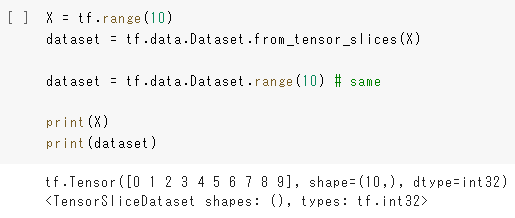
\includegraphics[width=200pt]{img/hands-on-ml_13-1_1.png}
    \end{column}
    \begin{column}[T]{0.4\mycolumnwidth}
      \centering
      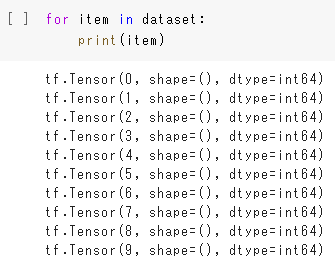
\includegraphics[width=110pt]{img/hands-on-ml_13-1_2.png}
    \end{column}
  \end{columns}

\end{frame}

%%%%%%%%%%%%%%%%%%%%%%%%%%%%%%%%%%%%%%%%%%%%%%%%%%

\hypertarget{ux5909ux63dbux306eux9023ux9396}{%
  \subsection{13.1.1 変換の連鎖}\label{ux5909ux63dbux306eux9023ux9396}}

%%%%%%%%%%%%%%%%%%%%%%%%%%%%%%%%%%%%%%%%%%%%%%%%%%

\begin{frame}{別のデータセットに変換するメソッド 1/4}\label{ux5225ux306eux30c7ux30fcux30bfux30bbux30c3ux30c8ux306bux5909ux63dbux3059ux308bux30e1ux30bdux30c3ux30c9-14}

  \begin{columns}[totalwidth=\mytotalwidth]
    \begin{column}[t]{0.75\mycolumnwidth}
      \begin{itemize}
        \tightlist
        \item
              repeat(n)

              \begin{itemize}
                \tightlist
                \item
                      \alert{1つのスライスをn回連結}
                \item
                      コピーではない(高速かつ小容量?)
              \end{itemize}
        \item
              batch(n)

              \begin{itemize}
                \tightlist
                \item
                      スライスを\alert{n個ずつのスライスに分割}
                \item
                      最後のバッチがn個未満の場合、\\
                      引数にdrop\_remainder=Trueで削除可能
              \end{itemize}
      \end{itemize}
    \end{column}

    \begin{column}[T]{0.25\mycolumnwidth}
      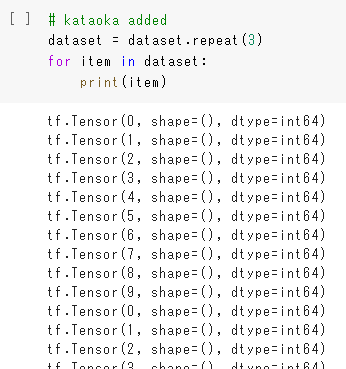
\includegraphics[width=110pt]{img/hands-on-ml_13-1-1_1.png}
      \\
      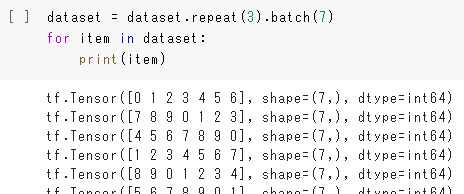
\includegraphics[width=110pt]{img/hands-on-ml_13-1-1_2.png}
    \end{column}
  \end{columns}

\end{frame}

%%%%%%%%%%%%%%%%%%%%%%%%%%%%%%%%%%%%%%%%%%%%%%%%%%

\begin{frame}{別のデータセットに変換するメソッド 2/4}\label{ux5225ux306eux30c7ux30fcux30bfux30bbux30c3ux30c8ux306bux5909ux63dbux3059ux308bux30e1ux30bdux30c3ux30c9-24}

  \begin{itemize}
    \tightlist
    \item
          \href{https://qiita.com/conf8o/items/0cb02bc504b51af09099}{map}(lambda
          x: xの式)

          \begin{itemize}
            \tightlist
            \item
                  \alert{要素をラムダ式で柔軟に変換する}など
            \item
                  TF関数に変換可能なラムダ式のみ対応(12章)
            \item
                  \href{https://tensorflow.classcat.com/2019/03/23/tf20-alpha-guide-data-performance/}{引数num\_parallel\_calls=tf.data.experimental.AUTOTUNEで\\並列化&高速化}
          \end{itemize}
  \end{itemize}
  \centering
  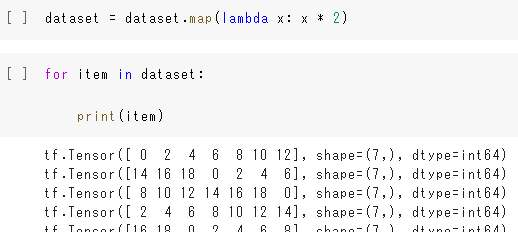
\includegraphics[width=200pt]{img/hands-on-ml_13-1-1_3.png}
\end{frame}

%%%%%%%%%%%%%%%%%%%%%%%%%%%%%%%%%%%%%%%%%%%%%%%%%%

\begin{frame}{別のデータセットに変換するメソッド 3/4}\label{ux5225ux306eux30c7ux30fcux30bfux30bbux30c3ux30c8ux306bux5909ux63dbux3059ux308bux30e1ux30bdux30c3ux30c9-34}

  \begin{itemize}
    \tightlist
    \item
          unbach()

          \begin{itemize}
            \tightlist
            \item
                  \alert{bach()で作ったデータセットを解体}
            \item
                  試験段階のメソッドで、collabではエラー
          \end{itemize}
    \item
          apply()

          \begin{itemize}
            \tightlist
            \item
                  \alert{{[}{]}で囲まれたデータセット全体に適用}
            \item
                  引数にdataset.unbach()などを用いる
          \end{itemize}
  \end{itemize}

  \centering
  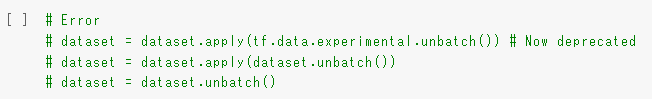
\includegraphics[width=300pt]{img/hands-on-ml_13-1-1_4.png}

\end{frame}

%%%%%%%%%%%%%%%%%%%%%%%%%%%%%%%%%%%%%%%%%%%%%%%%%%

\begin{frame}{別のデータセットに変換するメソッド 4/4}\label{ux5225ux306eux30c7ux30fcux30bfux30bbux30c3ux30c8ux306bux5909ux63dbux3059ux308bux30e1ux30bdux30c3ux30c9-44}

  \begin{itemize}
    \tightlist
    \item
          filter(lambda x: xを用いたbool演算)

          \begin{itemize}
            \tightlist
            \item
                  \alert{ラムダ式がtrueの要素xのみのスライスを返す}
          \end{itemize}
    \item
          take(n)

          \begin{itemize}
            \tightlist
            \item
                  \alert{先頭からn個の要素を用いる}
          \end{itemize}
  \end{itemize}

  \centering
  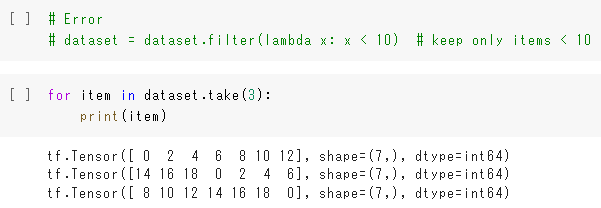
\includegraphics[width=230pt]{img/hands-on-ml_13-1-1_5.png}

\end{frame}

%%%%%%%%%%%%%%%%%%%%%%%%%%%%%%%%%%%%%%%%%%%%%%%%%%

\hypertarget{ux30c7ux30fcux30bfux306eux30b7ux30e3ux30c3ux30d5ux30eb}{%
  \subsection{13.1.2 データのシャッフル}\label{ux30c7ux30fcux30bfux306eux30b7ux30e3ux30c3ux30d5ux30eb}}

%%%%%%%%%%%%%%%%%%%%%%%%%%%%%%%%%%%%%%%%%%%%%%%%%%

\begin{frame}{Datasetのシャッフル 1/2}
  % \begin{wrapfigure}[4]{r}[0mm]{width=190pt}
  %   \centering
  %   \includegraphics[keepaspectratio,width=180pt]
  %   {img/hands-on-ml_13-1-2_1.png}
  % \end{wrapfigure}
  \begin{itemize}
    \tightlist
    \item shuffle(buffer\_size=n, seed=m)
          % shuffle(buffer\_size=n, seed=m)
          % \quad \backgroundsetup{scale=1, contents=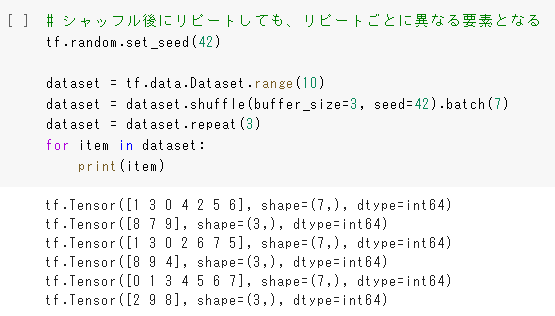
\includegraphics{img/hands-on-ml_13-1-2_1.png}}
          \begin{itemize}
            \tightlist
            \item
                  \alert{要素のシャッフル}
            \item
                  \alert{
                    独立同分布(同一の分布から独立に抽出された状態)でよく機能する勾配降下法などで使用
                  }
                  \textcolor{gray}{(4章)}
            \item
                  大規模なデータからサイズnのバッファを経由してシャッフル
            \item
                  大規模データセットに見合った大きいバッファサイズが必要
            \item
                  RAMの容量に注意
            \item
                  shuffle()後にrepeat(3)しても、3回とも異なるリピートとなる\textcolor{gray}{(次頁)}

                  \begin{itemize}
                    \tightlist
                    \item
                          引数reshuffle\_each\_iteration=Falseで同じリピートにできる
                  \end{itemize}
          \end{itemize}
  \end{itemize}

\end{frame}

%%%%%%%%%%%%%%%%%%%%%%%%%%%%%%%%%%%%%%%%%%%%%%%%%%

\begin{frame}{Datasetのシャッフル 2/2}

  \begin{columns}[totalwidth=\mytotalwidth]
    \begin{column}[T]{0.4\mycolumnwidth}
      \centering
      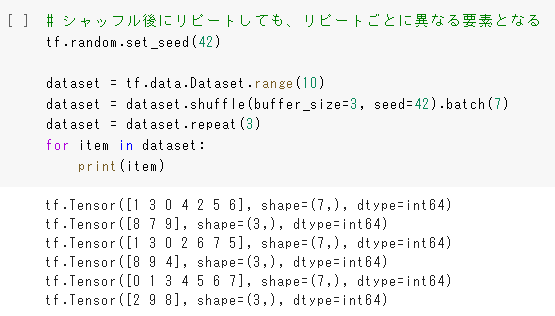
\includegraphics[width=160pt]{img/hands-on-ml_13-1-2_1.png}
    \end{column}

    \begin{column}[T]{0.6\mycolumnwidth}
      \centering
      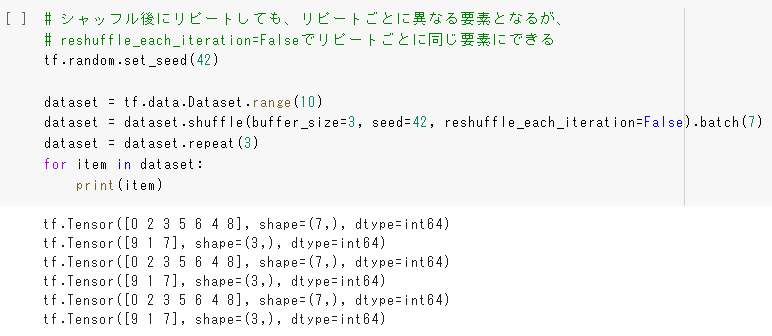
\includegraphics[width=240pt]{img/hands-on-ml_13-1-2_2.png}
    \end{column}
  \end{columns}


\end{frame}

%%%%%%%%%%%%%%%%%%%%%%%%%%%%%%%%%%%%%%%%%%%%%%%%%%

\begin{frame}{便利なシャッフル}

  \begin{itemize}
    \tightlist
    \item
          list\_files(DATA\_FILE\_PATH, seed=n)

          \begin{itemize}
            \tightlist
            \item
                  \alert{データをシャッフルしてから}ロード
            \item
                  引数suffle=Falseも指定可能
          \end{itemize}
    \item
          interleave(lambda file\_name: ラムダ式, cycle\_length=n)

          \begin{itemize}
            \tightlist
            \item
                  \alert{n個のファイルを同時に無作為に読み出す}
            \item
                  n個のデータセットをもつ1個のデータセットを作成
            \item
                  n個のデータセット間の同じ長さの部分が\alert{互い違い}になる

                  \begin{itemize}
                    \tightlist
                    \item
                          \href{https://tensorflow.classcat.com/2019/03/23/tf20-alpha-guide-data-performance/}{引数num\_parallel\_calls=tf.data.experimental.AUTOTUNEで初めて並列化する}
                  \end{itemize}
            \item
                  コードでは、ファイルパスが尽きるまで5個ずつ取り出して\\
                  インターリーブする操作を繰り返している
          \end{itemize}
  \end{itemize}

\end{frame}

%%%%%%%%%%%%%%%%%%%%%%%%%%%%%%%%%%%%%%%%%%%%%%%%%%

\hypertarget{ux30c7ux30fcux30bfux306eux524dux51e6ux7406}{%
  \subsection{13.1.3 データの前処理}\label{ux30c7ux30fcux30bfux306eux524dux51e6ux7406}}

%%%%%%%%%%%%%%%%%%%%%%%%%%%%%%%%%%%%%%%%%%%%%%%%%%

\begin{frame}{CSVデータのスケーリング}
  \begin{columns}[totalwidth=\mytotalwidth]
    \begin{column}[t]{0.75\mycolumnwidth}

      \begin{itemize}
        \tightlist
        \item
              TFで上手く平均0 分散1に統一したい
        \item
              tf.io.decode\_csv(LINE, record={[}\ldots{]})

              \begin{itemize}
                \tightlist
                \item
                      第1引数:CSVの1行
                \item
                      第2引数:1行の列数とデータ型がわかる\\
                      初期値を格納した配列

                      \begin{itemize}
                        \tightlist
                        \item
                              敢えて0.を入れると欠損時に例外を吐く
                      \end{itemize}
                \item
                      \alert{1レコードの1次元テンソル\\
                      {[}{[}\ldots{]}, \ldots, {[}\ldots{]}{]}を返す}

                      \begin{itemize}
                        \tightlist
                        \item
                              tf.stack(fields{[}スライス表現{]})で{[}\ldots,{]}に直す
                      \end{itemize}
              \end{itemize}
      \end{itemize}
    \end{column}

    \begin{column}[T]{0.25\mycolumnwidth}
      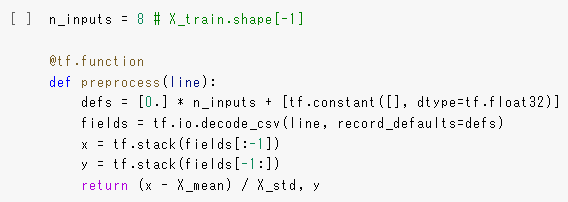
\includegraphics[width=140pt]{img/hands-on-ml_13-1-3_1.png}
    \end{column}
  \end{columns}

\end{frame}

%%%%%%%%%%%%%%%%%%%%%%%%%%%%%%%%%%%%%%%%%%%%%%%%%%

\hypertarget{ux3064ux306bux307eux3068ux3081ux308b}{%
  \subsection{13.1.4 1つにまとめる}\label{ux3064ux306bux307eux3068ux3081ux308b}}

%%%%%%%%%%%%%%%%%%%%%%%%%%%%%%%%%%%%%%%%%%%%%%%%%%

\begin{frame}{これまでの処理を関数化}

  \begin{itemize}
    \tightlist
    \item
          新要素は最後の行のprefetch(1)のみ\textcolor{gray}{(後述)}
  \end{itemize}

  \centering
  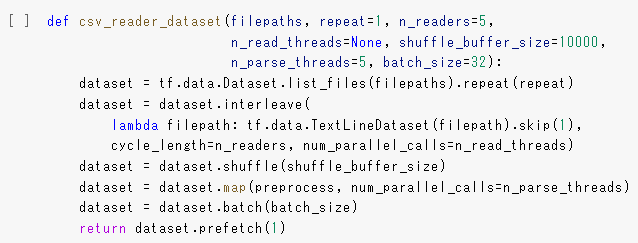
\includegraphics[width=400pt]{img/hands-on-ml_13-1-4_1.png}

\end{frame}

%%%%%%%%%%%%%%%%%%%%%%%%%%%%%%%%%%%%%%%%%%%%%%%%%%

\hypertarget{ux30d7ux30eaux30d5ux30a7ux30c3ux30c1}{%
  \subsection{13.1.5 プリフェッチ}\label{ux30d7ux30eaux30d5ux30a7ux30c3ux30c1}}

%%%%%%%%%%%%%%%%%%%%%%%%%%%%%%%%%%%%%%%%%%%%%%%%%%

\begin{frame}{プリフェッチによる並列化}

  \begin{columns}[totalwidth=\mytotalwidth]
    \begin{column}[t]{0.8\mycolumnwidth}

      \begin{itemize}
        \tightlist
        \item
              prefetch(n)

              \begin{itemize}
                \tightlist
                \item
                      \alert{n個のバッチをCPUとGPUで並列・高速化}
                \item
                      一般にn=1でよい
                \item
                      GPUのRAMの容量や帯域幅(速度)が重要
                \item
                      引数num\_parallel\_calls\\  =tf.data.experimental.AUTOTUNE

                      \begin{itemize}
                        \tightlist
                        \item
                              CPU内で並列化
                        \item
                              nを自動調節
                      \end{itemize}
              \end{itemize}
      \end{itemize}

    \end{column}
    \begin{column}[T]{0.20\mycolumnwidth}
      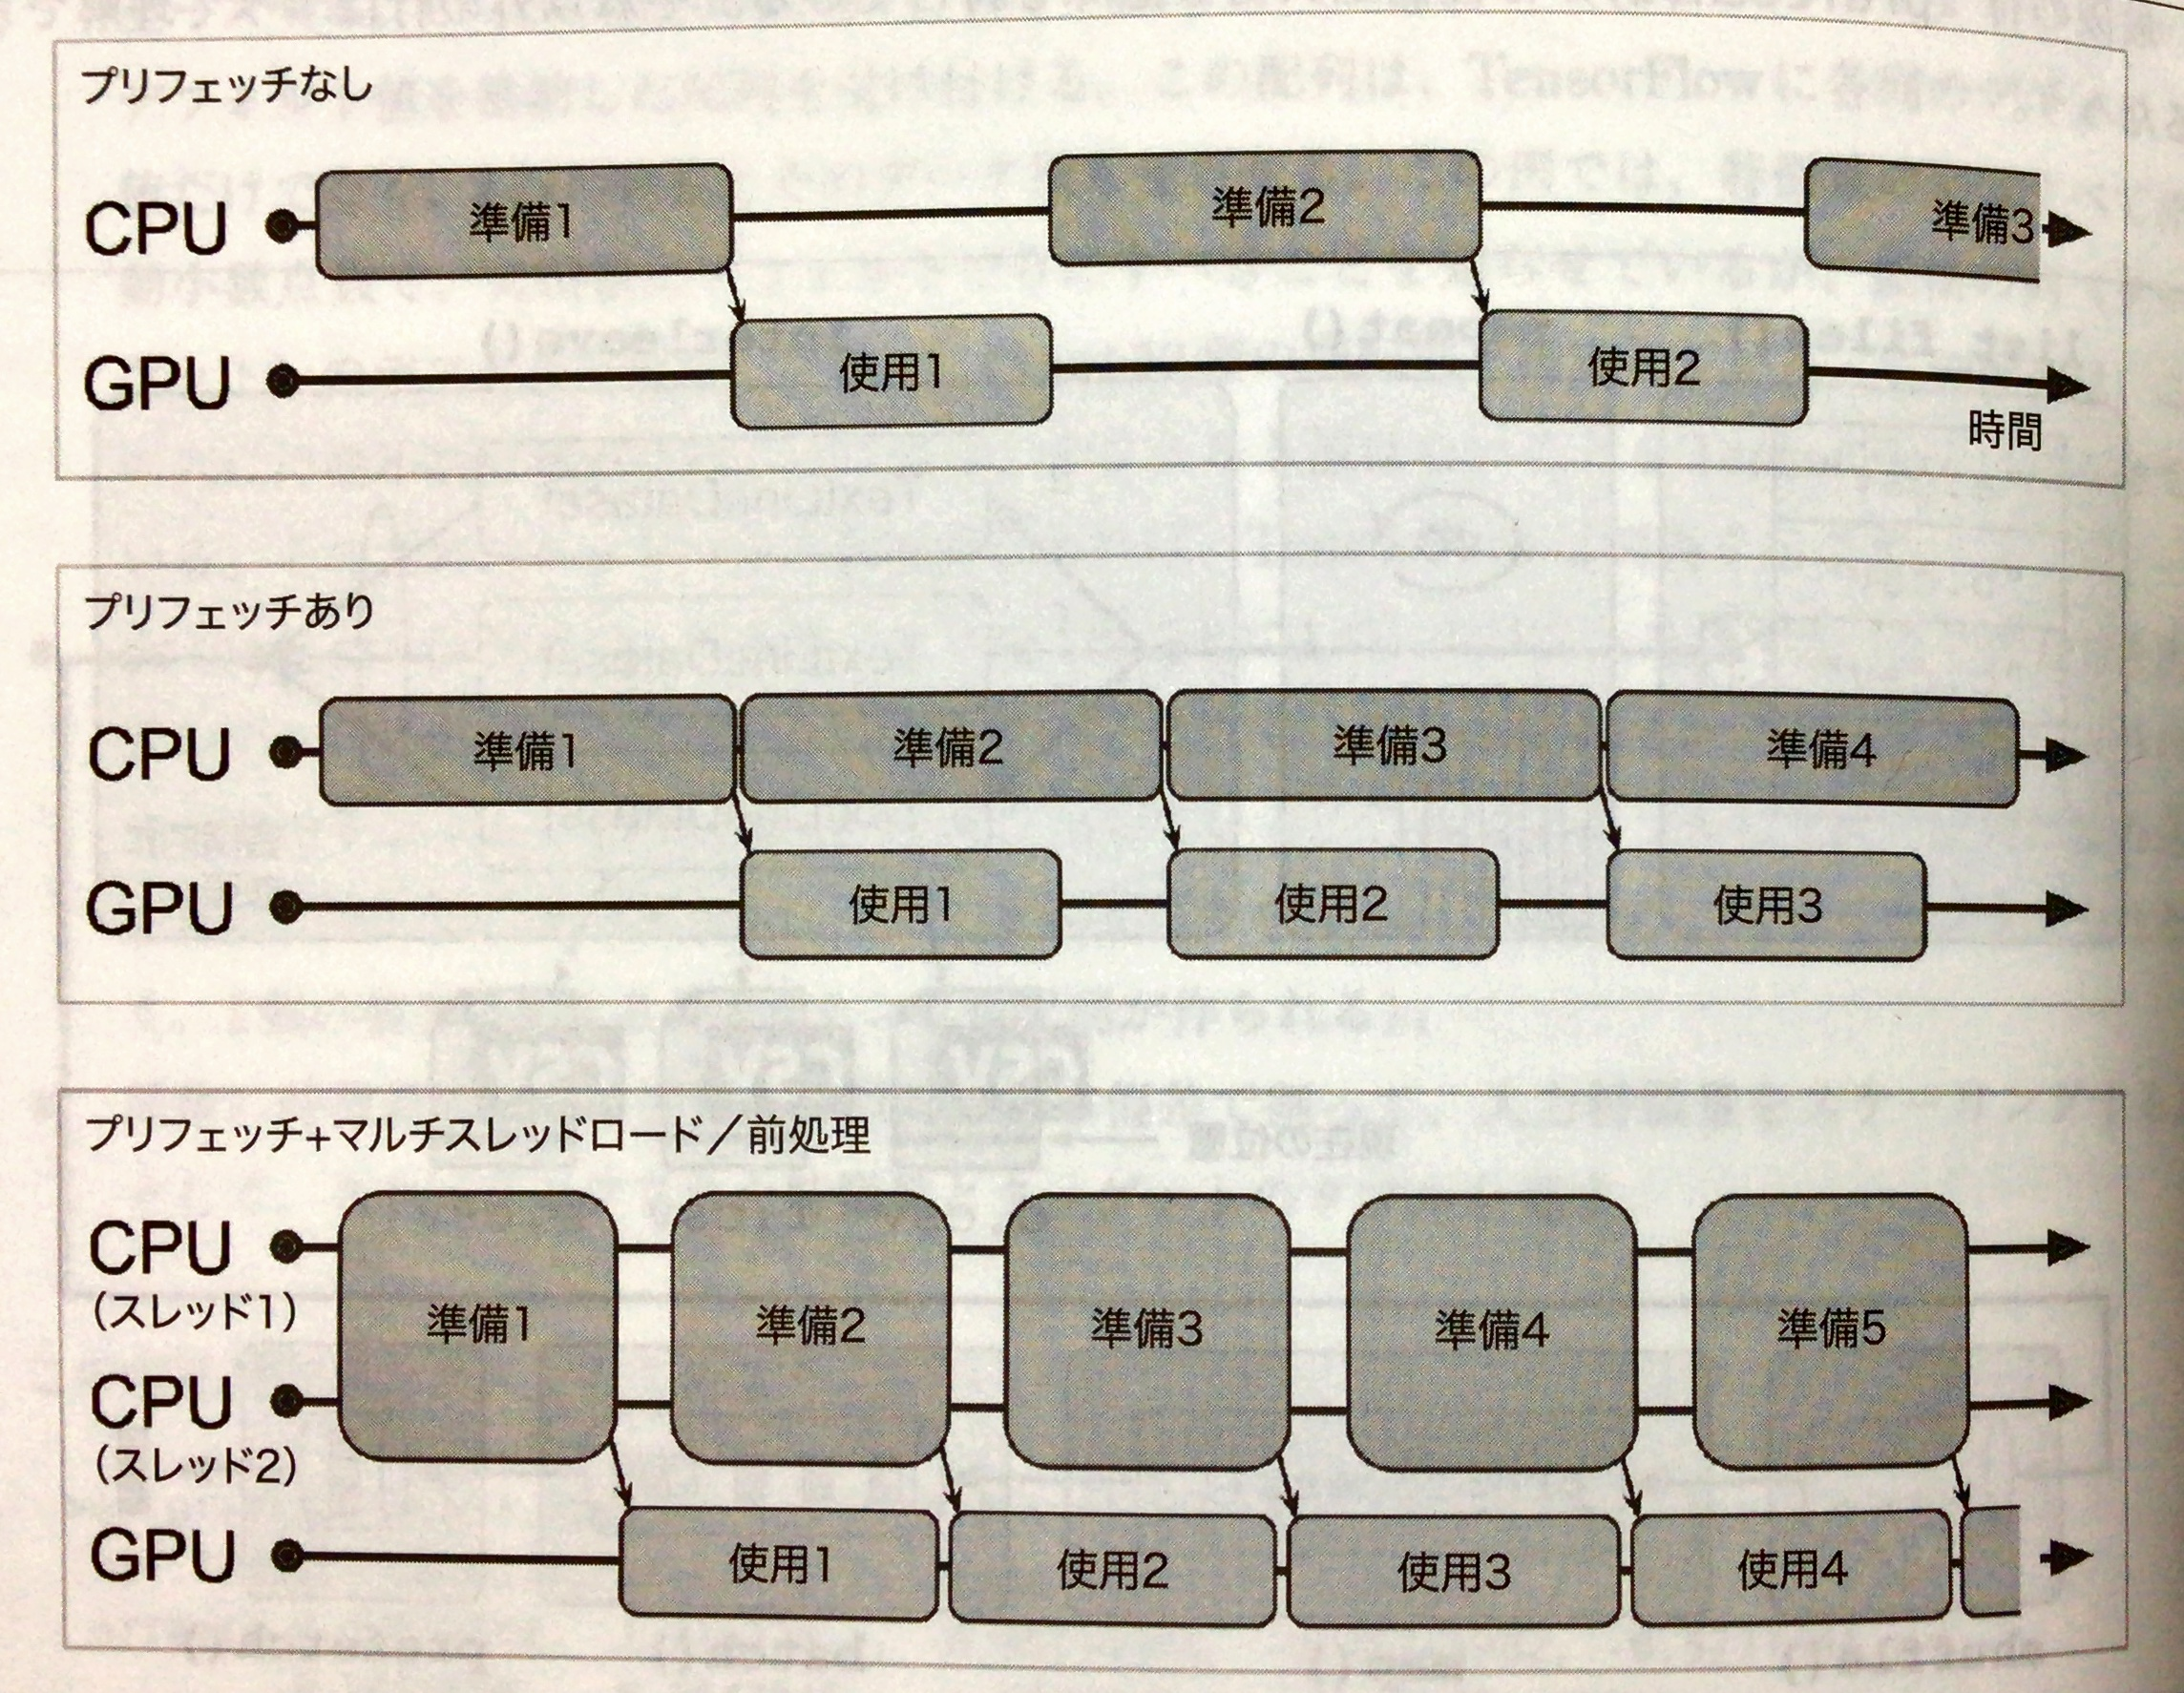
\includegraphics[width=125pt]{img/hands-on-ml_13-1-5_1.jpg}
    \end{column}
  \end{columns}

\end{frame}

%%%%%%%%%%%%%%%%%%%%%%%%%%%%%%%%%%%%%%%%%%%%%%%%%%

\begin{frame}{その他の便利な関数}
  \begin{columns}[totalwidth=\mytotalwidth]
    \begin{column}[t]{0.5\mycolumnwidth}
      \begin{itemize}
        \tightlist
        \item
              cache()

              \begin{itemize}
                \tightlist
                \item
                      データセットがメモリに入る程度に小さいときに高速化
                \item
                      ロード前処理とシャッフルの間で実行
              \end{itemize}
        \item
              concatenate()
        \item
              zip()
        \item
              window()
      \end{itemize}
    \end{column}
    \begin{column}[t]{0.5\mycolumnwidth}
      \begin{itemize}
        \item
              reduce()
        \item
              shard()\ \textcolor{gray}{ = 破片}
        \item
              flat\_map()
        \item
              padded\_batch()
        \item
              from\_generator()
        \item
              from\_tensors()
      \end{itemize}
    \end{column}
  \end{columns}

\end{frame}

%%%%%%%%%%%%%%%%%%%%%%%%%%%%%%%%%%%%%%%%%%%%%%%%%%

\hypertarget{tf.kerasux306eux3082ux3068ux3067ux306eux30c7ux30fcux30bfux30bbux30c3ux30c8ux306eux4f7fux3044ux65b9}{%
  \subsection{13.1.6 tf.kerasのもとでのデータセットの使い方}\label{tf.kerasux306eux3082ux3068ux3067ux306eux30c7ux30fcux30bfux30bbux30c3ux30c8ux306eux4f7fux3044ux65b9}}

%%%%%%%%%%%%%%%%%%%%%%%%%%%%%%%%%%%%%%%%%%%%%%%%%%

\begin{frame}{データセットの応用 1/3}

  \begin{itemize}
    \tightlist
    \item
          種々のデータセットの作成
  \end{itemize}

  \centering
  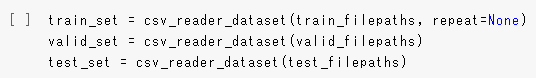
\includegraphics[width=240pt]{img/hands-on-ml_13-1-6_1.png}

\end{frame}

%%%%%%%%%%%%%%%%%%%%%%%%%%%%%%%%%%%%%%%%%%%%%%%%%%

\begin{frame}{データセットの応用 2/3}

  \begin{itemize}
    \tightlist
    \item
          モデルの構築と訓練
  \end{itemize}

  \centering
  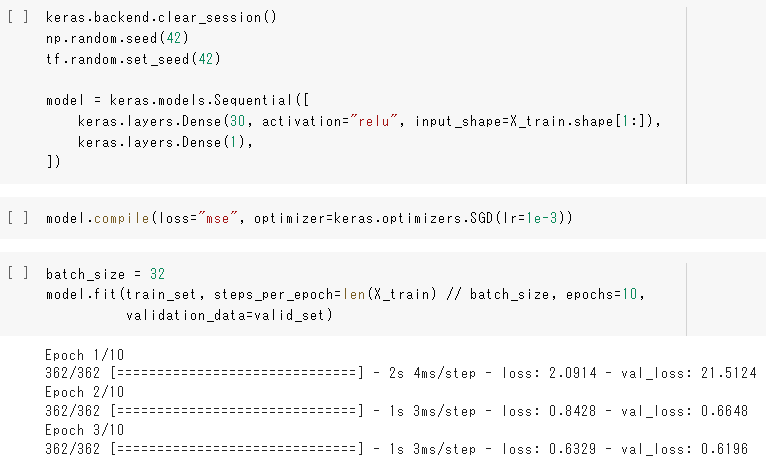
\includegraphics[width=240pt]{img/hands-on-ml_13-1-6_2.png}

\end{frame}

%%%%%%%%%%%%%%%%%%%%%%%%%%%%%%%%%%%%%%%%%%%%%%%%%%

\begin{frame}{データセットの応用 3/3}

  \begin{itemize}
    \tightlist
    \item
          テストの評価と新インスタンスの予測
  \end{itemize}

  \centering
  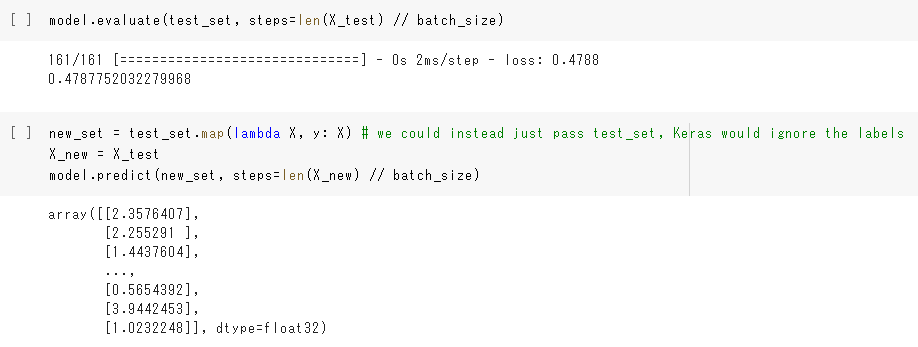
\includegraphics[width=240pt]{img/hands-on-ml_13-1-6_3.png}

\end{frame}

%%%%%%%%%%%%%%%%%%%%%%%%%%%%%%%%%%%%%%%%%%%%%%%%%%

\begin{frame}{独自のTF訓練関数(12章と同様)}

  \begin{itemize}
    \tightlist
    \item
          p,401の自動微分のコードと比較するとよい
  \end{itemize}

  \centering
  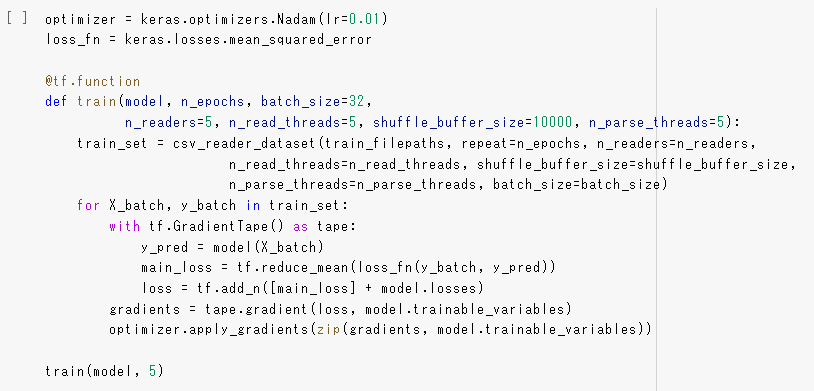
\includegraphics[height=170pt]{img/hands-on-ml_13-1-6_4.png}

\end{frame}

%%%%%%%%%%%%%%%%%%%%%%%%%%%%%%%%%%%%%%%%%%%%%%%%%%

\hypertarget{tfrecordux5f62ux5f0f}{%
  \section{13.2 TFRecord形式}\label{tfrecordux5f62ux5f0f}}

%%%%%%%%%%%%%%%%%%%%%%%%%%%%%%%%%%%%%%%%%%%%%%%%%%

\begin{frame}{TFRecord 概要}

  \begin{itemize}
    \tightlist
    \item
          TFデータのロードやパースがボトルネックなら用いる
    \item
          大規模なデータの効率的な格納・読み出しが可能
    \item
          可変長バイナリレコードのシーケンス

          \begin{itemize}
            \tightlist
            \item
                  長さ情報
            \item
                  長さ情報のCRCチェックサム
            \item
                  実データ
            \item
                  実データのチェックサム
          \end{itemize}
  \end{itemize}

\end{frame}

%%%%%%%%%%%%%%%%%%%%%%%%%%%%%%%%%%%%%%%%%%%%%%%%%%

\begin{frame}{TFRecordの利用}

  \begin{itemize}
    \tightlist
    \item
          書き込み\\
          \begin{center}
            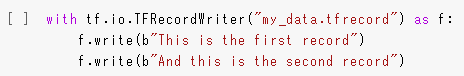
\includegraphics[width=240pt]{img/hands-on-ml_13-2_1.png}
          \end{center}
    \item
          読み出し・出力\\
          \begin{center}
            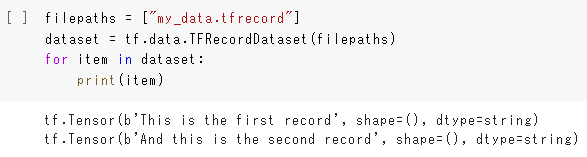
\includegraphics[width=240pt]{img/hands-on-ml_13-2_2.png}
          \end{center}
  \end{itemize}

\end{frame}

%%%%%%%%%%%%%%%%%%%%%%%%%%%%%%%%%%%%%%%%%%%%%%%%%%

\hypertarget{tfrecordux30d5ux30a1ux30a4ux30ebux306eux5727ux7e2e}{%
  \subsection{13.2.1 TFRecordファイルの圧縮}\label{tfrecordux30d5ux30a1ux30a4ux30ebux306eux5727ux7e2e}}

%%%%%%%%%%%%%%%%%%%%%%%%%%%%%%%%%%%%%%%%%%%%%%%%%%

\begin{frame}{TFRecordファイルの圧縮}

  \begin{columns}[totalwidth=\mytotalwidth]
    \begin{column}[t]{0.5\mycolumnwidth}
      \begin{itemize}
        \tightlist
        \item
              \alert{TFデータの送受信}に利用
        \item
              option引数で指定
        \item
              解凍
      \end{itemize}
    \end{column}

    \begin{column}[T]{0.5\mycolumnwidth}
      \centering
      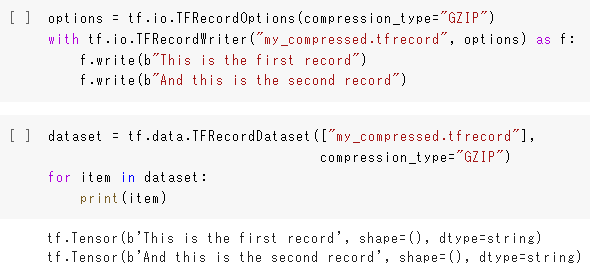
\includegraphics[width=200pt]{img/hands-on-ml_13-2-1_1.png}
    \end{column}

  \end{columns}

\end{frame}

%%%%%%%%%%%%%%%%%%%%%%%%%%%%%%%%%%%%%%%%%%%%%%%%%%

\hypertarget{ux30d7ux30edux30c8ux30b3ux30ebux30d0ux30c3ux30d5ux30a1ux5165ux9580}{%
  \subsection{13.2.2 プロトコルバッファ入門}\label{ux30d7ux30edux30c8ux30b3ux30ebux30d0ux30c3ux30d5ux30a1ux5165ux9580}}

%%%%%%%%%%%%%%%%%%%%%%%%%%%%%%%%%%%%%%%%%%%%%%%%%%

\begin{frame}{protobuf(プロトコルバッファ)}

  \begin{itemize}
    \tightlist
    \item
          通常のTFRecordで使われる\alert{シリアライズ化されたバイナリデータ}
    \item
          \alert{可搬性}と\alert{拡張性}に優れる
    \item
          protoc:protobufコンパイラ
    \item
          .protocファイル内の定義例
  \end{itemize}

  \centering
  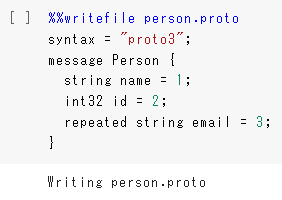
\includegraphics[height=100pt]{img/hands-on-ml_13-2-2_1.png}

\end{frame}

%%%%%%%%%%%%%%%%%%%%%%%%%%%%%%%%%%%%%%%%%%%%%%%%%%

\begin{frame}{Pythonのprotobufアクセスクラスの使用例}

  \begin{columns}[totalwidth=\mytotalwidth]
    \begin{column}[t]{0.5\mycolumnwidth}
      \begin{itemize}
        \tightlist
        \item
              personインスタンスの\\可視化や読み書き
        \item
              SerializeToString()で\\シリアライズ
        \item
              ParseFromString()で\\デシリアライズ
      \end{itemize}
    \end{column}

    \begin{column}[T]{0.5\mycolumnwidth}
      \centering
      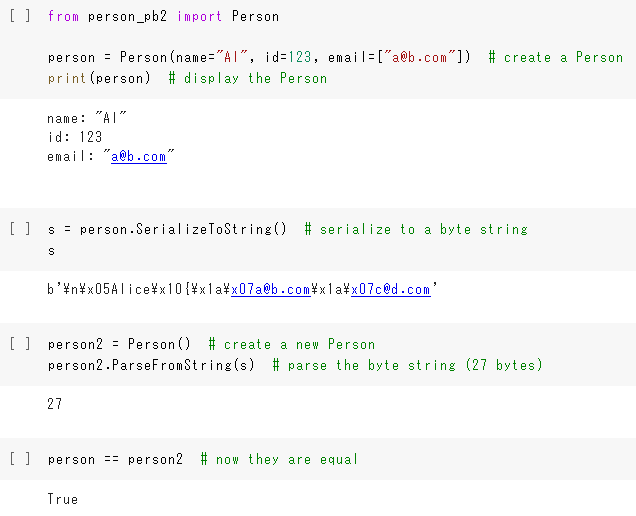
\includegraphics[width=200pt]{img/hands-on-ml_13-2-2_2.png}
    \end{column}

  \end{columns}

\end{frame}

%%%%%%%%%%%%%%%%%%%%%%%%%%%%%%%%%%%%%%%%%%%%%%%%%%

\begin{frame}{protobufとTFとの関係}

  \begin{itemize}
    \tightlist
    \item
          \alert{protocファイルで定義したクラスはTFオペレーションでない}

          \begin{itemize}
            \tightlist
            \item
                  TF関数に単純に組み込めない
            \item
                  tf.py\_function()で組み込むと速度と可搬性が落ちる
            \item
                  TFで定義された特別なprotobuf定義で解決する
          \end{itemize}
    \item
          その他詳細

          \begin{itemize}
            \tightlist
            \item
                  https://developers.google.com/protocol-buffers/
          \end{itemize}
  \end{itemize}

\end{frame}

%%%%%%%%%%%%%%%%%%%%%%%%%%%%%%%%%%%%%%%%%%%%%%%%%%

\end{document}
